\section{Pippo Francfrog}\label{pippo-francfrog}

Tags: PC Alias: La Rana Esplosiva Creatore: Francesco G. Giocatore:
Francesco Gabrielli Ispirazione: Pippo Franco Luogo: Kos Razza: Frogfolk
Classe: Artificiere Livello: 10

\section{Pippo Francfrog}\label{pippo-francfrog-1}

\begin{center}\rule{0.5\linewidth}{0.5pt}\end{center}

\begin{figure}
\centering
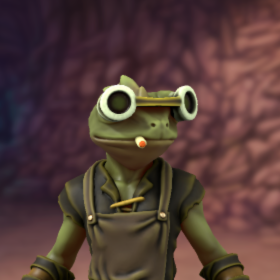
\includegraphics{Pippo_Francfrog-Token.png}
\caption{Pippo Francfrog-Token.png}
\end{figure}

Informazioni Generali

Età:

Anno di nascita:

Paese di nascita:

Razza: Frogfolk

Relazioni:

Alleati:

Nemesi:

Possedimenti importanti:

\begin{center}\rule{0.5\linewidth}{0.5pt}\end{center}

\subsection{1. Descrizione Generale}\label{descrizione-generale}

\begin{center}\rule{0.5\linewidth}{0.5pt}\end{center}

\begin{figure}
\centering
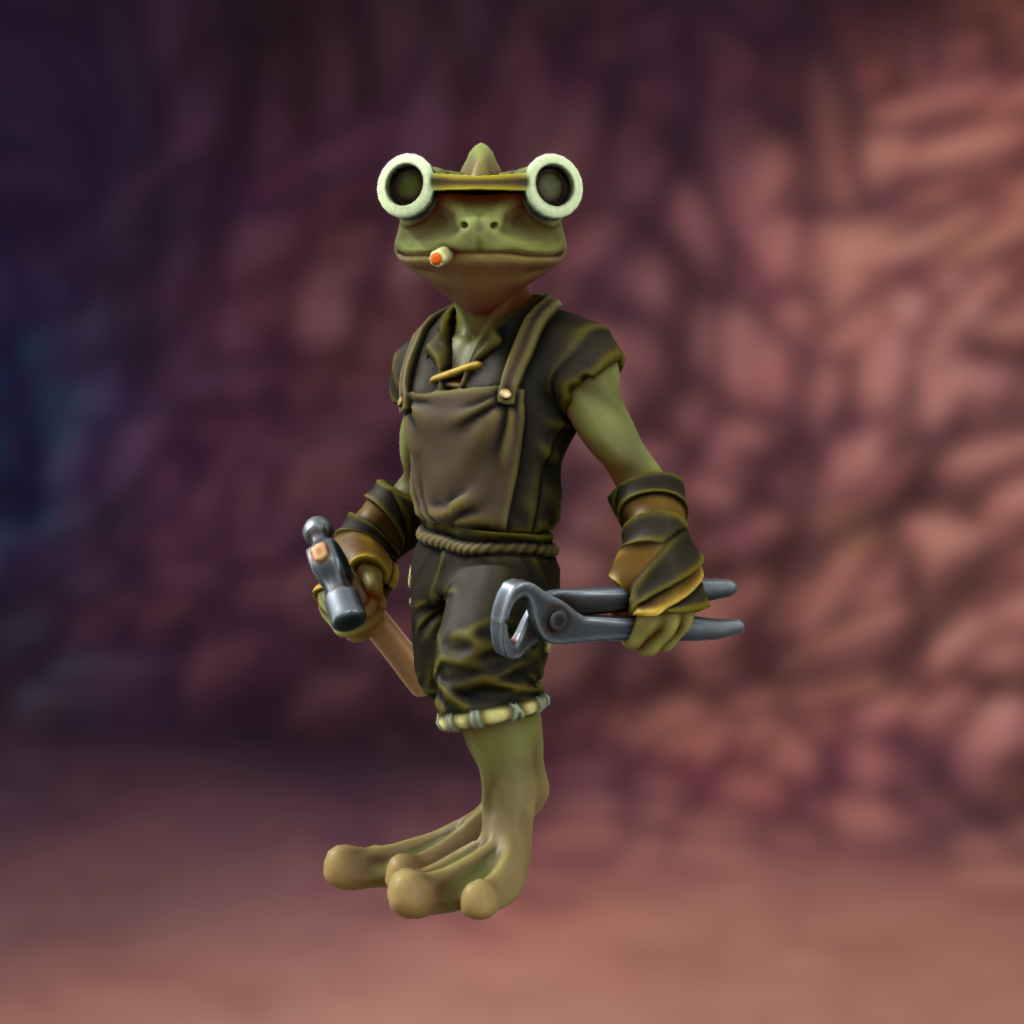
\includegraphics{Pippo_Francfrog-portrait.png}
\caption{Pippo Francfrog-portrait.png}
\end{figure}

Pippo Francfrog incarna l'incantevole fusione di una rana umanoide e la
magia dell'intrattenimento. La sua pelle iridescente rivela radici
anfibie, mentre lo sguardo intelligente brilla di carisma. Con abiti
vivaci e un sorriso contagioso, Pippo attrae l'attenzione ovunque vada.
La sua natura di artista si riflette in ogni gesto, mantenendo viva la
luce del palcoscenico anche mentre esplora nuovi orizzonti.

\begin{quote}
``Torte in faccia!''
\end{quote}

\subsection{2. Biografia}\label{biografia}

\begin{center}\rule{0.5\linewidth}{0.5pt}\end{center}

\subsubsection{2.1 Infanzia e le Origini
Mistiche}\label{infanzia-e-le-origini-mistiche}

Pippo Francfrog vide la luce grazie a un incantesimo complesso e ardito
lanciato dal mago Lasalmadi Mikebongiorno. La sua creazione era un
tentativo di fondere la magia con il mondo dell'intrattenimento,
producendo così una creatura unica nel suo genere. Sin dalla sua
nascita, Pippo ha portato con sé un legame con la magia che avrebbe
influenzato il corso della sua vita.

\subsubsection{\texorpdfstring{2.2 \textbf{Esordi in ``Il
Bagaglione''}}{2.2 Esordi in ``Il Bagaglione''}}\label{esordi-in-il-bagaglione}

I primi passi di Pippo nel mondo dell'intrattenimento li compì entrando
a far parte dello spettacolo itinerante de ``Il Bagaglione''. Qui, Pippo
fu introdotto all'arte dell'intrattenimento e imparò i segreti
dell'interazione con il pubblico. Le sue performance coinvolgenti e
innovative catturarono l'attenzione di tutti coloro che ebbero la
fortuna di assistere ai suoi numeri.

\subsubsection{\texorpdfstring{2.3 \textbf{Richiamo della Magia e il
Percorso come
Artificiere}}{2.3 Richiamo della Magia e il Percorso come Artificiere}}\label{richiamo-della-magia-e-il-percorso-come-artificiere}

Mentre il suo talento nel campo dell'intrattenimento si faceva sempre
più evidente, la sua connessione con la magia iniziò a emergere in modo
più preponderante. Sentendo il richiamo della magia dentro di sé, Pippo
intraprese un nuovo cammino come artificiere. La sua abilità nel creare
oggetti incantati e invenzioni uniche gli permise di esprimere la sua
creatività in modi mai sperimentati prima.

\subsubsection{\texorpdfstring{2.4 \textbf{Unione Fraterna con Pippo
Baudog}}{2.4 Unione Fraterna con Pippo Baudog}}\label{unione-fraterna-con-pippo-baudog}

Le avventure di Pippo non furono mai solitarie. Insieme a suo fratello
Pippo Baudog, un cane antropomorfo con il medesimo retaggio magico,
intraprese molte imprese. La loro partnership rappresentava l'armoniosa
fusione tra intrattenimento e abilità magica, dimostrando il valore
dell'affetto fraterno nel raggiungimento dei traguardi.

\subsubsection{\texorpdfstring{2.5 \textbf{Eredità e
Impatto}}{2.5 Eredità e Impatto}}\label{eredituxe0-e-impatto}

La vita di Pippo Francfrog è rimasta una testimonianza dell'incrocio tra
il mondo della magia e dell'intrattenimento. La sua biografia incarna la
perseveranza nella ricerca della propria passione, nonostante le diverse
sfaccettature della sua identità. La sua eredità continua a ispirare
coloro che cercano di fondere passioni divergenti, aprendo la strada a
un mondo di meraviglia, sorpresa e collaborazione.

\subsection{3. Carriera}\label{carriera}

\begin{center}\rule{0.5\linewidth}{0.5pt}\end{center}

La carriera di Pippo Francfrog è stata un connubio straordinario tra
magia e intrattenimento. Dopo esordi di successo con lo spettacolo
itinerante de ``Il Bagaglione'', Pippo ha seguito il richiamo della
magia e si è dedicato all'artigianato magico come artificiere.
Nonostante questo cambiamento di percorso, non ha mai dimenticato le sue
radici da intrattenitore, portando sempre con sé il desiderio di
incantare e stupire il pubblico. Collaborando spesso con suo fratello,
Pippo Baudog, ha dimostrato come la fusione di talento e creatività
possa creare un'esperienza unica e indimenticabile per chiunque lo
incontri. La sua carriera è un esempio di come diverse passioni possano
coesistere e arricchirsi a vicenda, creando un mondo di meraviglia e
sorpresa.

\subsection{4. Personalità}\label{personalituxe0}

\begin{center}\rule{0.5\linewidth}{0.5pt}\end{center}

La personalità di Pippo Francfrog è un affascinante mix di carisma,
curiosità e creatività. È un individuo straordinariamente affabile, con
un sorriso contagioso e uno sguardo che riflette un'intelligenza
brillante. La sua natura di intrattenitore è evidente in ogni aspetto
della sua vita, portando con sé l'abilità di incantare e stupire
chiunque incontri. La sua curiosità insaziabile lo spinge a esplorare
nuovi orizzonti, sia nell'arte dello spettacolo che nell'artigianato
magico. Tuttavia, il suo cuore rimane fedele al desiderio di portare
gioia e meraviglia al pubblico, e questa passione è il motore che guida
ogni sua azione. La sua personalità è un richiamo costante alla magia
della creatività e all'importanza di diffondere la gioia attraverso
l'arte e lo spettacolo.

\subsection{5. Coinvolgimenti in eventi
recenti}\label{coinvolgimenti-in-eventi-recenti}

\begin{center}\rule{0.5\linewidth}{0.5pt}\end{center}

\href{Untitled\%20Database\%2035b391282a354aefb762c6cbe4670abc.csv}{Untitled
Database}

\subsection{6. Scheda personaggio}\label{scheda-personaggio}

\begin{center}\rule{0.5\linewidth}{0.5pt}\end{center}

\href{Info\%20PG\%2075172870926b4488a518a676f6c59d30.csv}{Info PG}

\subsubsection{Statistiche e abilità}\label{statistiche-e-abilituxe0}

\begin{center}\rule{0.5\linewidth}{0.5pt}\end{center}

\href{Abilita\%CC\%80\%206c389f50c35f46369e8056828b53fcb0.csv}{Abilità}

\subsubsection{Lista magie}\label{lista-magie}

\subsection{A. Descrizione originale}\label{a.-descrizione-originale}

\begin{center}\rule{0.5\linewidth}{0.5pt}\end{center}

Pippo Francfrog, una rana umanoide, e suo fratello Pippo Baudog, un cane
antropomorfo, erano creature uniche nel loro genere. Creati dal mago
Lasalmadi Mikebongiorno con l'ambizioso scopo di diventare i conduttori
televisivi più talentuosi mai visti, i due fratelli avevano ciascuno una
strada differente da percorrere. Fin da giovane, Pippo Baudog dimostrò
un carisma naturale e una passione per l'intrattenimento. Il suo talento
era innegabile, e presto divenne il conduttore di spicco della Sagra
della Canzone di Sam Reno, conducendo con maestria numerose edizioni
dell'evento amato da tutti. Dall'altra parte, Pippo Francfrog si unì
allo spettacolo itinerante de ``Il Bagaglione''. Durante il periodo
trascorso con il collettivo, Pippo Francfrog imparò l'arte
dell'intrattenimento e si esibiva con il suo vecchio gruppo in numeri
coinvolgenti e straordinari. Tuttavia, il richiamo della sua natura da
artificiere divenne sempre più forte. Così, dopo un certo periodo di
successo con ``Il Bagaglione'', Pippo Francfrog decise di seguire la sua
vera passione e si dedicò alla professione di artificiere. La creazione
di oggetti magici e invenzioni uniche gli permise di esprimere il suo
talento creativo e di utilizzare la sua innata abilità nella magia.
Nonostante la sua scelta, Pippo Francfrog non dimenticò mai le sue
origini da conduttore. Durante le avventure che intraprendeva insieme a
Pippo Baudog e il loro gruppo di compagni, o insieme a nuovi compagni,
non esitava a riproporre alcuni dei suoi vecchi numeri, portando ancora
una volta gioia e stupore ai suoi spettatori. Pippo Francfrog e Pippo
Baudog continuarono insieme a vivere saltuariamente avventure
emozionanti, unendo le loro abilità uniche per affrontare sfide e
pericoli. L'amore fraterno che li legava era indissolubile, e il loro
rapporto di collaborazione e sostegno reciproco li rese una coppia
imbattibile.
